\documentclass{vkr}
\usepackage[english, russian]{babel} % переносы
\usepackage{graphicx} % для вставки картинок
\graphicspath{{images/}} % путь к изображениям
\usepackage[hidelinks]{hyperref}
\usepackage{float} % определяет метод H для рисунка с переносом на следующую страницу, ели не помещается
\usepackage{pdflscape}
\addto{\captionsrussian}{\renewcommand{\refname}{СПИСОК ИСПОЛЬЗОВАННЫХ ИСТОЧНИКОВ}}
\usepackage{xltabular} % для вставки таблиц
\usepackage{makecell}
\renewcommand\theadfont{} % шрифт в /thead
\usepackage{array} % для определения новых типов столбцов таблиц
\newcolumntype{T}{>{\centering\arraybackslash}X} % новый тип столбца T - автоматическая ширина столбца с выравниванием по центру
\newcolumntype{R}{>{\raggedleft\arraybackslash}X} % новый тип столбца R - автоматическая ширина столбца с выравниванием по правому краю
\newcolumntype{C}[1]{>{\centering\let\newline\\\arraybackslash\hspace{0pt}}m{#1}} % новый тип столбца C - фиксированная ширина столбца с выравниванием по центру
\newcolumntype{r}[1]{>{\raggedleft\arraybackslash}p{#1}} % новый тип столбца r - фиксированная ширина столбца с выравниванием по правому краю
\newcommand{\centrow}{\centering\arraybackslash} % командой \centrow можно центрировать одну ячейку (заголовок) в столбце типа X или p, оставив в оcтальных ячейках другой тип выравнивания
\newcommand{\finishhead}{\endhead\hline\endlastfoot}
\newcommand{\continuecaption}[1]{\caption*{#1}\\ \hline }
\usepackage{etoolbox}
\AtBeginEnvironment{xltabular}{\refstepcounter{tablecnt}} % подсчет таблиц xltabular, обычные таблицы подсчитываются в классе

\usepackage[tableposition=top]{caption} % подпись таблицы вверху
\captionsetup{strut=off}
\setlength{\intextsep}{0pt} % Vertical space above & below [h] floats
\setlength{\textfloatsep}{0pt} % Vertical space below (above) [t] ([b]) floats
\DeclareCaptionLabelFormat{gostfigure}{Рисунок #2} %подпись рисунка
\DeclareCaptionLabelFormat{gosttable}{Таблица #2} %подпись таблицы
\DeclareCaptionLabelSeparator{gost}{~--~} %разделитель в рисунках и таблицах
\captionsetup{labelsep=gost}
\captionsetup[figure]{aboveskip=10pt,belowskip=4mm,justification=centering,labelformat=gostfigure} % настройка подписи рисунка
\captionsetup[table]{font={stretch=1.41},skip=0pt,belowskip=0pt,aboveskip=8.5pt,singlelinecheck=off,labelformat=gosttable} % настройка подписи таблицы

\setlength{\LTpre}{8mm} % отступ сверху таблицы
\setlength{\LTpost}{6mm} % отступ снизу таблицы

\usepackage{enumitem}
\setlist{nolistsep,wide=\parindent,itemindent=*} % отступы вокруг списков, выравнивание с учетом разделителя

\usepackage{color} %% это для отображения цвета в коде
\usepackage{listings} %% листинги кода
\setmonofont[Scale=0.7]{Verdana} % моноширный шрифт для листинга

\definecolor{codegreen}{rgb}{0,0.6,0}
\definecolor{codegray}{rgb}{0.5,0.5,0.5}
\definecolor{codepurple}{rgb}{0.58,0,0.82}

\lstset{ %
language=C,                 % выбор языка для подсветки (здесь это С)
numbers=left,               % где поставить нумерацию строк (слева\справа)
numberstyle=\tiny,           % размер шрифта для номеров строк
stepnumber=1,                   % размер шага между двумя номерами строк
numbersep=5pt,                % как далеко отстоят номера строк от подсвечиваемого кода
commentstyle=\color{codegreen},
keywordstyle=\color{magenta},
numberstyle=\tiny\color{codegray},
stringstyle=\color{codepurple},
basicstyle=\linespread{0.95}\ttfamily,
backgroundcolor=\color{white}, % цвет фона подсветки - используем \usepackage{color}
showspaces=false,            % показывать или нет пробелы специальными отступами
showstringspaces=false,      % показывать или нет пробелы в строках
showtabs=false,             % показывать или нет табуляцию в строках
frame=single,              % рисовать рамку вокруг кода
tabsize=2,                 % размер табуляции по умолчанию равен 2 пробелам
captionpos=t,              % позиция заголовка вверху [t] или внизу [b] 
breaklines=true,           % автоматически переносить строки (да\нет)
breakatwhitespace=false, % переносить строки только если есть пробел
escapeinside={\%*}{*)}   % если нужно добавить комментарии в коде
}

\makeatletter % чтобы допускались русские комментарии в листингах
\lst@InputCatcodes
\def\lst@DefEC{%
 \lst@CCECUse \lst@ProcessLetter
  ^^80^^81^^82^^83^^84^^85^^86^^87^^88^^89^^8a^^8b^^8c^^8d^^8e^^8f%
  ^^90^^91^^92^^93^^94^^95^^96^^97^^98^^99^^9a^^9b^^9c^^9d^^9e^^9f%
  ^^a0^^a1^^a2^^a3^^a4^^a5^^a6^^a7^^a8^^a9^^aa^^ab^^ac^^ad^^ae^^af%
  ^^b0^^b1^^b2^^b3^^b4^^b5^^b6^^b7^^b8^^b9^^ba^^bb^^bc^^bd^^be^^bf%
  ^^c0^^c1^^c2^^c3^^c4^^c5^^c6^^c7^^c8^^c9^^ca^^cb^^cc^^cd^^ce^^cf%
  ^^d0^^d1^^d2^^d3^^d4^^d5^^d6^^d7^^d8^^d9^^da^^db^^dc^^dd^^de^^df%
  ^^e0^^e1^^e2^^e3^^e4^^e5^^e6^^e7^^e8^^e9^^ea^^eb^^ec^^ed^^ee^^ef%
  ^^f0^^f1^^f2^^f3^^f4^^f5^^f6^^f7^^f8^^f9^^fa^^fb^^fc^^fd^^fe^^ff%
  ^^^^20ac^^^^0153^^^^0152%
  % Basic Cyrillic alphabet coverage
  ^^^^0410^^^^0411^^^^0412^^^^0413^^^^0414^^^^0415^^^^0416^^^^0417%
  ^^^^0418^^^^0419^^^^041a^^^^041b^^^^041c^^^^041d^^^^041e^^^^041f%
  ^^^^0420^^^^0421^^^^0422^^^^0423^^^^0424^^^^0425^^^^0426^^^^0427%
  ^^^^0428^^^^0429^^^^042a^^^^042b^^^^042c^^^^042d^^^^042e^^^^042f%
  ^^^^0430^^^^0431^^^^0432^^^^0433^^^^0434^^^^0435^^^^0436^^^^0437%
  ^^^^0438^^^^0439^^^^043a^^^^043b^^^^043c^^^^043d^^^^043e^^^^043f%
  ^^^^0440^^^^0441^^^^0442^^^^0443^^^^0444^^^^0445^^^^0446^^^^0447%
  ^^^^0448^^^^0449^^^^044a^^^^044b^^^^044c^^^^044d^^^^044e^^^^044f%
  ^^^^0401^^^^0451%
  %%%
  ^^00}
\lst@RestoreCatcodes
\makeatother


% Режим шаблона (должен быть включен один из трех)
\Курсоваяtrue

\newcommand{\Дисциплина}{<<Проектирование и архитектура программных систем>>} % для курсовой
\newcommand{\КодСпециальности}{09.03.04} % Курсовая
\newcommand{\Специальность}{Программная инженерия} % Курсовая
\newcommand{\Тема}{Разработка web-сайта «LeCourses-онлайн магазин курсов» } % ВКР Курсовая
\newcommand{\ТемаВтораяСтрока}{}
\newcommand{\ГдеПроводитсяПрактика}{Юго-Западном государственном университете} % для практики
\newcommand{\РуководительПрактПредпр}{Куркина А. В.} % для практики
\newcommand{\ДолжнРуководительПрактПредпр}{директор} % для практики
\newcommand{\РуководительПрактУнивер}{Чаплыгин А. А.} % для практики
\newcommand{\ДолжнРуководительПрактУнивер}{к.т.н. доцент} % для практики
\newcommand{\Автор}{И. А. Седых}
\newcommand{\АвторРод}{Седых И.А.}
\newcommand{\АвторПолностьюРод}{Седых Ивана Александровича} % для практики
\newcommand{\Шифр}{21-06-0028}
\newcommand{\Курс}{3} % для практики
\newcommand{\Группа}{ПО-11б}
\newcommand{\Руководитель}{А. А. Чаплыгин} % для ВКР и курсовой
\newcommand{\Нормоконтроль}{А. А. Чаплыгин} % для ВКР
\newcommand{\ЗавКаф}{А. В. Малышев} % для ВКР
\newcommand{\ДатаПриказа}{«07» апреля 2023~г.} % для ВКР
\newcommand{\НомерПриказа}{1505-с} % для ВКР
\newcommand{\СрокПредоставления}{«24» января 2024~г.} % для ВКР, курсового

\begin{document}
\maketitle
\ifПрактика{}\else{
   \newpage
\begin{center}
\large\textbf{Минобрнауки России}

\large\textbf{Юго-Западный государственный университет}
\vskip 1em
\normalsize{Кафедра программной инженерии}
\vskip 1em
\ifВКР{
        \begin{flushright}
        \begin{tabular}{p{.4\textwidth}}
        \centrow УТВЕРЖДАЮ: \\
        \centrow Заведующий кафедрой \\
        \hrulefill \\
        \setarstrut{\footnotesize}
        \centrow\footnotesize{(подпись, инициалы, фамилия)}\\
        \restorearstrut
        «\underline{\hspace{1cm}}»
        \underline{\hspace{3cm}}
        20\underline{\hspace{1cm}} г.\\
        \end{tabular}
        \end{flushright}
        }\fi
\end{center}
\vspace{1em}
  \begin{center}
  \large
\ifВКР{
ЗАДАНИЕ НА ВЫПУСКНУЮ КВАЛИФИКАЦИОННУЮ РАБОТУ
  ПО ПРОГРАММЕ БАКАЛАВРИАТА}
  \else
ЗАДАНИЕ НА КУРСОВУЮ РАБОТУ (ПРОЕКТ)
\fi
\normalsize
  \end{center}
\vspace{1em}
{\parindent0pt
  Студента \АвторРод, шифр\ \Шифр, группа \Группа
  
1. Тема «\Тема\ \ТемаВтораяСтрока»
\ifВКР{
утверждена приказом ректора ЮЗГУ от \ДатаПриказа\ № \НомерПриказа
}\fi.

2. Срок предоставления работы к защите \СрокПредоставления

3. Исходные данные для создания программной системы:

3.1. Перечень решаемых задач:}

\renewcommand\labelenumi{\theenumi)}

\begin{enumerate}
\item проанализировать ситуацию на рынке онлайн-курсов;
\item разработать концептуальную модель магазина на основе анализа конкурентов;
\item спроектировать программу онлайн-магазина;
\item сконструировать и протестировать программу онлайн-магазина.
\end{enumerate}

{\parindent0pt
  3.2. Входные данные и требуемые результаты для программы:}

\begin{enumerate}
\item Входными данными для программной системы являются: данные
справочников комплектующих, конфигураций, ПО, критериев качества SLA,
ИТ-услуг, департаментов компании; технические данные ИТ-ресурсов; данные входящих заявок на ИТ-ресурсы; данные запросов поставщикам на комплектующие.
\item Выходными данными для программной системы являются: сформированные заявки на обслуживание ИТ-ресурсов; сформированные запросы на
закупку комплектующих; сведения о выполненных работах по заявкам; статусы заявок; выходные отчеты (инфографика) – по качеству услуг, по состоянию ИТ-ресурсов, по деятельности ИТ-отдела, по стоимости обслуживания
ИТ-ресурсов, воронка заявок.
\end{enumerate}

{\parindent0pt

  4. Содержание работы (по разделам):
  
  4.1. Введение
  
  4.1. Анализ предметной области
  
4.2. Техническое задание: основание для разработки, назначение разработки,
требования к программной системе, требования к оформлению документации.

4.3. Технический проект: общие сведения о программной системе, проект
данных программной системы, проектирование архитектуры программной системы, проектирование пользовательского интерфейса программной системы.

4.4. Рабочий проект: спецификация компонентов и классов программной системы, тестирование программной системы, сборка компонентов программной системы.

4.5. Заключение

4.6. Список использованных источников

5. Перечень графического материала:

\списокПлакатов

\vskip 2em
\begin{tabular}{p{6.8cm}C{3.8cm}C{4.8cm}}
Руководитель \ifВКР{ВКР}\else работы (проекта) \fi & \lhrulefill{\fill} & \fillcenter\Руководитель\\
\setarstrut{\footnotesize}
& \footnotesize{(подпись, дата)} & \footnotesize{(инициалы, фамилия)}\\
\restorearstrut
Задание принял к исполнению & \lhrulefill{\fill} & \fillcenter\Автор\\
\setarstrut{\footnotesize}
& \footnotesize{(подпись, дата)} & \footnotesize{(инициалы, фамилия)}\\
\restorearstrut
\end{tabular}
}

\renewcommand\labelenumi{\theenumi.}

   \abstract{РЕФЕРАТ}

Объем работы равен \formbytotal{lastpage}{страниц}{е}{ам}{ам}. Работа содержит \formbytotal{figurecnt}{иллюстраци}{ю}{и}{й}, \formbytotal{tablecnt}{таблиц}{у}{ы}{}, \arabic{bibcount} библиографических источников. Количество приложений – 1. Фрагменты исходного кода представлены в приложении А.

Перечень ключевых слов: сайт курсов, веб-сайт, контакты, профиль, пользователь, оплата, описание курсов, цена курса.

Объектом разработки веб-сайта магазина курсов является создание современной, функциональной онлайн-платформы, предназначенной для продажи и предоставления образовательных курсов.

Целью выпускной квалификационной работы по созданию сайта курсов заключается в разработке полнофункционального и эффективного веб-сайта, предназначенного для предоставления образовательных курсов. Работа направлена на продемонстрирование навыков проектирования и разработки веб-приложения, а также способности создать удобное пространство для предоставления и управления курсами, обеспечивая пользовательский комфорт и функциональность.

В процессе создания сайта были выделены основные сущности путем создания информационных блоков, использованы классы и методы модулей, обеспечивающие работу с сущностями предметной области, а также корректную работу web-сайта, разработаны разделы, содержащие страницу курсов, информацию о сайте, обратной связи, покупки курсов.


\selectlanguage{english}
\abstract{ABSTRACT}
  
The volume of work is \formbytotal{lastpage}{page}{}{s}{s}. The work contains \formbytotal{figurecnt}{illustration}{}{s}{s}, \formbytotal{tablecnt}{table}{}{s}{s}, \arabic{bibcount} bibliographic sources. The number of applications is 1. The layout of the site, including the connection of components, is presented in annex A.

List of keywords: course website, website, contacts, profile, user, payment, course description, course price.

The object of development for the online course store website is to create a modern, functional online platform designed for the sale and provision of educational courses.

The aim of the final qualification project for creating a course website is to develop a fully functional and effective website designed to provide educational courses. The work is aimed at demonstrating skills in designing and developing a web application, as well as the ability to create a convenient space for offering and managing courses, ensuring user comfort and functionality.

During the website creation process, the main entities were identified by creating informational blocks. Classes and methods of modules were used to handle entities in the subject area and ensure the correct functioning of the website. Sections were developed, including the course page, information about the website, feedback, and course purchase.
\selectlanguage{russian}
}\fi
\tableofcontents
\section*{ОБОЗНАЧЕНИЯ И СОКРАЩЕНИЯ}

БД -- база данных.

ИС -- информационная система.

ИТ -- информационные технологии. 

КТС -- комплекс технических средств.

ОМТС -- отдел материально-технического снабжения. 

ПО -- программное обеспечение.

РП -- рабочий проект.

СУБД -- система управления базами данных.

ТЗ -- техническое задание.

ТП -- технический проект.

UML (Unified Modelling Language) -- язык графического описания для объектного моделирования в области разработки программного обеспечения.

\ifПрактика{}\else{\section*{ВВЕДЕНИЕ}
\addcontentsline{toc}{section}{ВВЕДЕНИЕ}

В современном информационном обществе, под воздействием стремительного развития технологий, образование приобретает новые измерения. Студенты и профессионалы ищут удобные и эффективные способы обучения, а интернет становится неотъемлемой частью этого процесса. В этом контексте, онлайн-образование приобретает все большую популярность, а онлайн магазины курсов выступают важным звеном в современной образовательной парадигме.

Цель данной курсовой работы — исследовать и проанализировать концепцию онлайн магазина курсов, рассмотреть его преимущества и вызовы, а также выявить влияние данного формата образования на процесс обучения и доступ к знаниям. Путем анализа существующих платформ и тенденций в данной области, мы стремимся глубже понять, как онлайн магазины курсов взаимодействуют с современной образовательной средой и в чем заключаются их основные особенности.

Развитие технологий и их влияние на образование предоставляют уникальные возможности для инноваций в обучении. Онлайн магазины курсов являются проявлением этих изменений, предоставляя гибкость и доступность обучения, которые ранее казались невозможными. В нашей работе мы попытаемся рассмотреть различные аспекты этого феномена, выявить его преимущества и недостатки, а также оценить перспективы развития онлайн образования через призму онлайн магазинов курсов.

Главной задачей профессионально построенного сайта является превращение посетителя, зашедшего на сайт, в потенциального клиента.

\emph{Цель настоящей работы} – разработка web-сайта онлайн-магазина для привлечения новой аудитории, увеличения заказов, рекламы продукции и услуг компании. Для достижения поставленной цели необходимо решить \emph{следующие задачи:}
\begin{itemize}
\item провести анализ предметной области;
\item разработать концептуальную модель web-сайта;
\item спроектировать web-сайт;
\item реализовать сайт средствами web-технологий.
\end{itemize}

\emph{Структура и объем работы.} Отчет состоит из введения, 4 разделов основной части, заключения, списка использованных источников, 1 приложения. Текст выпускной квалификационной работы равен \formbytotal{page}{страниц}{е}{ам}{ам}.

\emph{Во введении} сформулирована цель работы, поставлены задачи разработки, описана структура работы, приведено краткое содержание каждого из разделов.

\emph{В первом разделе} на стадии описания технической характеристики предметной области приводится сбор информации о деятельности компании, для которой осуществляется разработка сайта.

\emph{Во втором разделе} на стадии технического задания приводятся требования к разрабатываемому сайту.

\emph{В третьем разделе} на стадии технического проектирования представлены проектные решения для web-сайта.

\emph{В четвертом разделе} приводится список классов и их методов, использованных при разработке сайта, производится тестирование разработанного сайта.

В заключении излагаются основные результаты работы, полученные в ходе разработки.

В приложении А представлены фрагменты исходного кода. 
}\fi
\section{Анализ предметной области}
\subsection{Исследование рынка онлайн-образования.}

В современном образовательном ландшафте онлайн магазины курсов представляют собой значительное изменение в том, как люди получают знания и развивают свои профессиональные навыки. Этот раздел посвящен более глубокому анализу предметной области, охватывая ключевые аспекты функционирования онлайн магазинов курсов и их влияние на образовательные процессы.

1. Развитие онлайн образования: тенденции и динамика

Первоначальный взлет онлайн образования произошел в контексте постоянного роста технологических возможностей. Эволюция интернета и цифровых технологий обеспечила создание разнообразных онлайн платформ, предлагающих курсы по самым разным предметам. Важным аспектом этой тенденции является расширение доступа к образованию, снижение географических барьеров и предоставление возможности для обучения в удобное время.

2. Преимущества онлайн магазинов курсов

Анализируя функционал онлайн магазинов курсов, мы обращаем внимание на их преимущества. Гибкость в выборе предметов, доступность 24/7, индивидуальный темп обучения и множество форматов обучения — все эти факторы делают онлайн курсы привлекательными для разнообразных аудиторий, начиная от студентов до профессионалов, стремящихся обновить свои знания.

3. Вызовы и перспективы

Неоспоримые преимущества онлайн магазинов курсов сопровождаются вызовами. Отсутствие физической интеракции, проблемы с оценкой студенческого прогресса и необходимость постоянного обновления контента — все это становится объектом внимания образовательных исследований. Однако, несмотря на эти вызовы, онлайн магазины курсов имеют перспективы дальнейшего развития, особенно в условиях постоянно меняющегося мира труда.
\newpage
4. Влияние на традиционное образование

Интересен также вопрос о влиянии онлайн магазинов курсов на традиционные образовательные учреждения. Как они адаптируются к конкуренции, предлагают ли свои курсы в онлайн формате, и какие изменения происходят в подходах к обучению в классе?

Все эти аспекты предметной области требуют более детального анализа для полного понимания того, как онлайн магазины курсов становятся неотъемлемой частью современной образовательной экосистемы. Дальнейшее исследование позволит выявить тенденции, прогнозировать будущие изменения и предоставить практические рекомендации для улучшения качества образования в онлайн формате.
\subsection{Технологии и инструменты для разработки веб-сайта}

При выборе технологий и инструментов для разработки веб-сайта, многое зависит от конкретных требований проекта, его масштаба, функциональности, уровня безопасности, и доступности ресурсов. 

Python для серверной части:

Python - универсальный язык программирования, который широко используется для веб-разработки. Он предоставляет множество фреймворков (например, Django, Flask), а также может быть использован для написания серверной логики без использования фреймворков.

CSS и JS для верстки:

CSS (Cascading Style Sheets) и JavaScript являются основными технологиями для создания стилей и добавления интерактивности на веб-страницах. Их сочетание обеспечивает красивый и функциональный пользовательский интерфейс.
Отсутствие фреймворка:

Иногда написание приложения без использования фреймворка может быть полезным, особенно для простых проектов или для того, чтобы полностью контролировать структуру и логику вашего приложения.

Waitress для обслуживания:

Waitress - это легковесный веб-сервер для Python, который может использоваться для обслуживания ваших веб-приложений. Он часто используется для разработки и тестирования.

MySQL Workbench для базы данных:

MySQL Workbench - это инструмент администрирования баз данных MySQL, который предоставляет графический интерфейс для создания, редактирования и управления базами данных.
Ваш выбор технологий обеспечивает хорошую основу для разработки веб-приложений. Важно также учитывать требования проекта, его масштаб и будущую масштабируемость при выборе технологий.

\section{Техническое задание}
\subsection{Основание для разработки}

Основанием для разработки программы является задание на курсовую работу по дисциплине «Проектирование и архитектура программных систем» на тему «Разработка web-сайта «LeCourses-онлайн магазин курсов»»

\subsection{Цель и назначение разработки}

Основной задачей курсовой работы является разработка программы web-сайта онлайн магазина курсов.

Посредством создания конечной программы планируется устранить существующие проблемы в поиске курсов по программированию в интернете.

Задачами данной разработки являются:
\begin{itemize}
	\item создание интерфейса программы для пользователя;
	\item создание информационных разделов сайта;
	\item реализация формы для обратной связи;
	\item реализация формы для покупки курса;
	\item реализация добавления товара на сайт.
\end{itemize}

\subsection{Требования пользователя к интерфейсу программы}

Программа должна включать в себя:
\begin{itemize}
	\item навигацию по разделам;
	\item доступ для пользователя;
	\item покупку курса;
	\item авторизацию.
\end{itemize}

Композиция шаблона сайта представлена на рисунке ~\ref{плакат1:image}.

\begin{figure}[ht]
	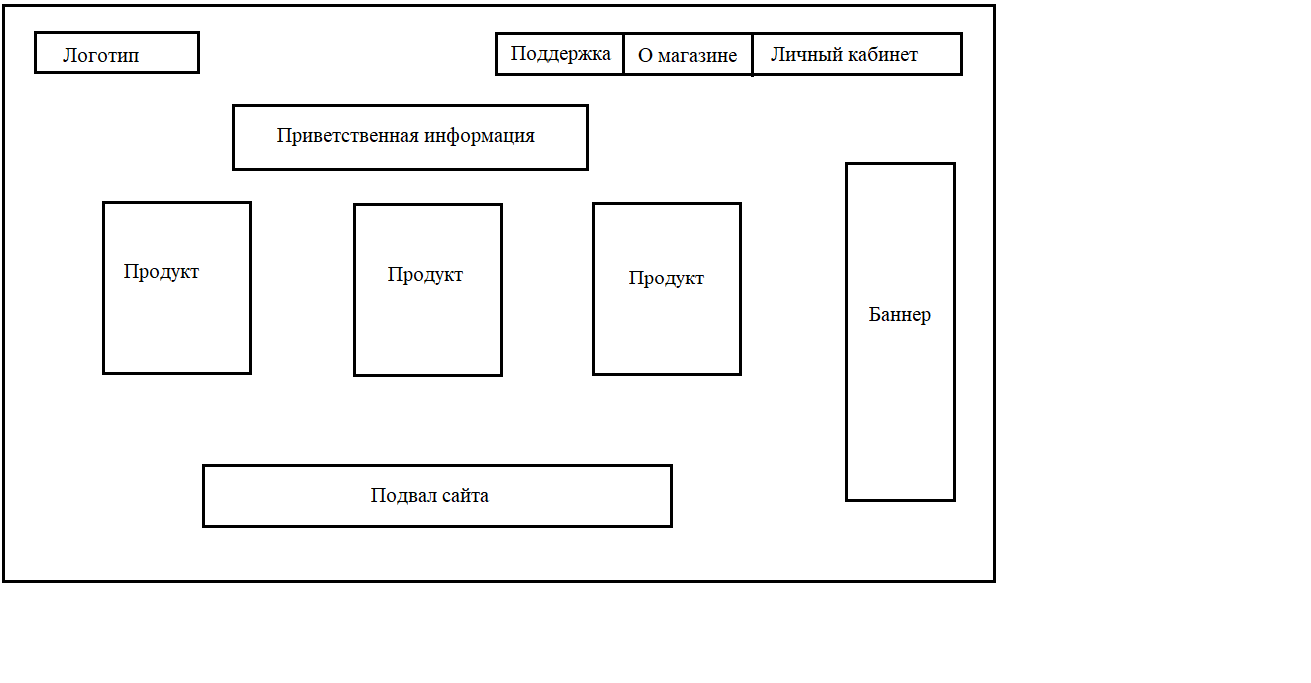
\includegraphics[width=1\linewidth]{плакат1}
	\caption{Композиция шаблона программы}
	\label{плакат1:image}
\end{figure}
%\vspace{-\figureaboveskip} % двойной отступ не нужен (можно использовать, если раздел заканчивается картинкой)

\subsection{Моделирование вариантов использования}

Для разрабатываемой программы была реализована модель, которая обеспечивает наглядное представление вариантов использования сайта.

Она помогает в физической разработке и детальном анализе взаимосвязей объектов. При построении диаграммы вариантов использования применяется унифицированный язык визуального моделирования UML.

Диаграмма вариантов описывает функциональное назначение разрабатываемой системы. То есть это то, что система будет непосредственно делать в процессе своего функционирования. Она является исходным концептуальным представлением системы в процессе ее проектирования и разработки. Проектируемая система представляется в виде ряда прецедентов, предоставляемых системой актерам или сущностям, которые взаимодействуют с системой. Актером или действующим лицом является сущность, взаимодействующая с системой извне (например, человек, техническое устройство). Прецедент служит для описания набора действий, которые система предоставляет актеру.

На основании анализа предметной области в программе должны быть реализованы следующие прецеденты:
\begin{enumerate}
	\item просмотр информации о сайте;
	\item регистрация пользователя;
	\item реализация обратной связи;
	\item просмотр информации о курсе;
	\item покупка курса.
\end{enumerate}

Диаграмма вариантов использования сайта представлена на рисунке ~\ref{прецедент:image}.

\begin{figure}[ht]
	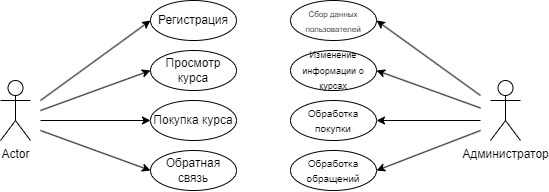
\includegraphics[width=1\linewidth]{прецедент}
	\caption{Прецеденты}
	\label{прецедент:image}
\end{figure}

\subsection{Требования к оформлению документации}

Разработка программной документации и программного изделия должна производиться согласно ГОСТ 19.102-77 и ГОСТ 34.601-90. Единая система программной документации.

\section{Технический проект}
\subsection{Общая характеристика организации решения задачи}

Необходимо спроектировать и разработать сайт, который должен способствовать успешной продаже курсов по программированию.

Интернет-сайт представляет собой набор взаимосвязанных электронных страниц, которые сгруппированы по разделам, содержащие текстовую, графическую, а также мультимедийную информацию (изображения и пр.). Сайт располагается в Интернете по определенному адресу – доменному имени сайта в виде www.имя\_сайта.ru. Каждая страница web-сайта – это текстовый документ, написанный на языке программирования (HTML, CSS, JavaScript и т.д.).

\subsection{Обоснование выбора технологии проектирования}

На сегодняшний день информационный рынок, поставляющий программные решения в выбранной сфере, предлагает множество продуктов, позволяющих достигнуть поставленной цели – разработки web-сайта.

\subsubsection{Описание используемых технологий и языков программирования}

В процессе разработки web-сайта используются программные средства и языки программирования. Каждое программное средство и каждый язык программирования применяется для круга задач, при решении которых они необходимы.

\subsubsection{Язык программирования Python}

Python – высокоуровневый язык программирования общего назначения с динамической строгой типизацией и автоматическим управлением памятью, ориентированный на повышение производительности разработчика, читаемости кода и его качества, а также на обеспечение переносимости написанных на нём программ. Использование Python позволило мне легко и эффективно разрабатывать серверную часть проекта, обеспечивая стабильную работу и высокую производительность.

\subsubsection{Язык программирования HTML}

Для разработки клиентской части проекта и отображения информации для пользователей, я использовал язык разметки HTML (HyperText Markup Language). HTML - это стандартный язык, используемый для создания веб-страниц, и он играет ключевую роль во взаимодействии пользователей с моим сервером.

Вот некоторые из основных плюсов HTML:
Простота и доступность: HTML - это язык разметки, который легко учить и использовать. 

Универсальность: HTML поддерживается практически всеми браузерами и устройствами, что позволяет создавать веб-страницы, доступные для широкой аудитории.

Семантика: HTML предоставляет разнообразные элементы и атрибуты для описания структуры и содержания веб-страницы. 

Версионная совместимость: HTML постоянно развивается, и новые версии (например, HTML5) включают в себя новые возможности и элементы. Это обеспечивает совместимость с более ранними версиями HTML и позволяет использовать современные функции.


\subsubsection{Язык программирования JavaScript}

JavaScript является ключевым языком для разработки клиентской части веб-приложений. Вот почему я выбрал JavaScript:

Интерактивность и динамичность: JavaScript позволяет создавать динамичные и интерактивные пользовательские интерфейсы. Это включает в себя асинхронное взаимодействие с сервером и изменение содержимого страницы без ее перезагрузки.

Широкая поддержка в браузерах: JavaScript поддерживается практически всеми современными браузерами, что обеспечивает высокую степень переносимости кода.

Возможности асинхронного программирования: JavaScript поддерживает асинхронный код, что особенно важно при работе с операциями ввода/вывода, такими как запросы к серверу или обработка событий.

Быстрое выполнение в браузере: JIT-компиляция в современных браузерах позволяет JavaScript выполняться достаточно быстро, что особенно важно для обеспечения быстрого отклика интерфейса.

\subsubsection{Язык разметки CSS}

CSS используется для оформления и стилизации веб-страниц. Вот почему я выбрал CSS:

Отделение структуры и стиля: CSS позволяет разделять структуру HTML и ее визуальное оформление, что упрощает обслуживание и обновление кода.

Множество возможностей стилизации: CSS предоставляет широкий набор возможностей для стилизации, включая цвета, шрифты, размеры, позиционирование и анимации.

\subsection{Диаграмма взаимодействия и схема обмена данными между представлениями}

Диаграмма взаимодействия описывает особенности физического представления разрабатываемой системы. Она позволяет определить архитектуру системы, установив зависимости между программными представлениями, в роли которых может выступать как исходный, так и исполняемый код. Основными графическими элементами диаграммы взаимодействия являются представлениями, интерфейсы, а также зависимости между ними. На рисунке \ref{comp:image} изображена диаграмма представлениями для проектируемой системы. Она включает в себя сервер с операционной системой, на которой установлена система управления содержимым, включающая в себя базу данных и интерфейс. Помимо этого на диаграмме изображен клиентский компьютер с операционной системой, на которой установлен браузер.

\begin{figure}[ht]
\center{\includegraphics[width=1\linewidth]{comp}}
\caption{Диаграмма компонентов}
\label{comp:image}
\end{figure}

Любое представление должно быть вызвано в сценарии страницы web-сайта. Web-страница передает данные представления в момент вызова последнего.

На рисунке \ref{представления:image} представлена схема обмена данными между сценариями представления при вызове представления на странице сайта.

\begin{figure}[ht]
\center{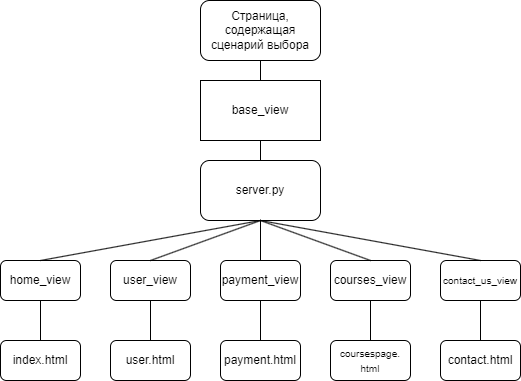
\includegraphics[width=1\linewidth]{представления}}
\caption{Диаграмма представления}
\label{представления:image}
\end{figure}

В файле server.py написан код, который представляет собой простое веб-приложение на Python, использующее фреймворк WSGI (Web Server Gateway Interface).

Здесь импортируются различные библиотеки, классы и функции, которые используются в приложении, такие как CGI, Waitress для веб-сервера, различные представления (views) и функции для работы с файлами и базой данных. Словарь urls соотносит URL-пути с соответствующими представлениями. Когда приходит запрос, код использует этот словарь для определения, какой обработчик использовать для данного URL. Основная функция app обрабатывает POST запрос для загрузки файла, извлекает данные из формы, вставляет изображение в БД и возвращает ответ в формате JSON. Обработка GET запроса происходит с логики определения и вызова соответствующего представления и логики для обработки статических файлов, определение MIME-типа и кодировки для ответа, а также установка заголовков ответа и возврат данных в ответе.

\subsection{Диаграмма размещения}

Диаграмма размещения (рис.~\ref{place:image}) отражает физические взаимосвязи между методами и представлениями.

\vspace{-8mm} % чтобы убрать пустую строку, которая осталась после переноса рисунка на следующую страницу
\begin{figure}[ht]
\center{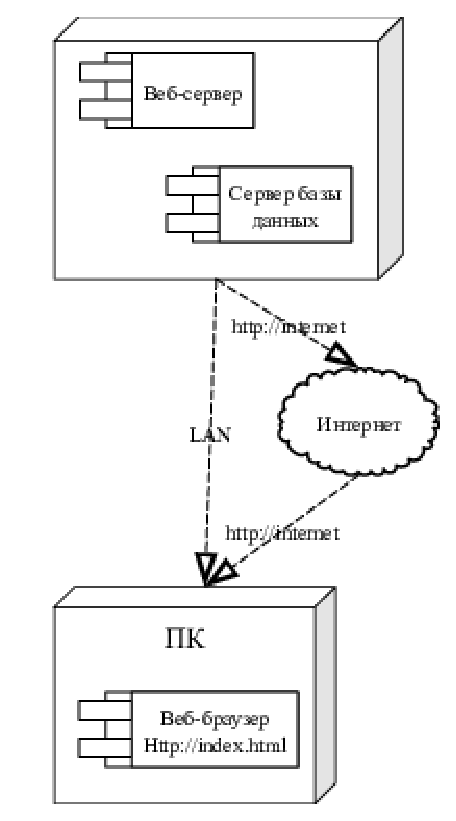
\includegraphics[width=0.57\linewidth]{place}}
\caption{Диаграмма размещения}
\label{place:image}
\end{figure}

Она является хорошим средством для показа маршрутов перемещения объектов и компонентов в распределенной системе.

\subsection{Содержание информационных блоков. Основные сущности}

Проанализировав требования, можно выделить две основных сущности:
\begin{itemize}
	\item "<Пользователь">;
	\item "<Покупка курса">;
\end{itemize}

В состав сущности "<Пользователь"> можно включить атрибуты, представленные в таблице 3.1.

\begin{xltabular}{\textwidth}{|l|l|p{1.7cm}|X|}
	\caption{Атрибуты сущности "<Пользователь">\label{news:table}}\\ \hline
	\centrow Поле & \centrow Тип & \centrow Обяза\-тельное & \centrow Описание \\ \hline
	\thead{1} & \thead{2} & \centrow 3 & \centrow 4 \\ \hline
	\endfirsthead
	\thead{1} & \thead{2} & \centrow 3 & \centrow 4 \\ \hline
	\finishhead
	id & ObjectId & true & Уникальный идентификатор \\ \hline 
	login & String & true & Логин \\ \hline 
	pass & String & true & Пароль \\ \hline 
\end{xltabular}

В состав сущности "<Покупка курса"> можно включить атрибуты, представленные в таблице 3.2.

\begin{xltabular}{\textwidth}{|l|l|p{1.7cm}|X|}
	\caption{Атрибуты сущности "<Покупка курса">\label{news:table}}\\ \hline
	\centrow Поле & \centrow Тип & \centrow Обяза\-тельное & \centrow Описание \\ \hline
	\thead{1} & \thead{2} & \centrow 3 & \centrow 4 \\ \hline
	\endfirsthead
	\thead{1} & \thead{2} & \centrow 3 & \centrow 4 \\ \hline
	\finishhead
	id & ObjectId & true & Уникальный идентификатор \\ \hline 
	name & String & true & Название курса \\ \hline 
	cost & Integer & true & Цена курса \\ \hline 
	description & String & true & Уровень сложности \\ \hline 
	about & String & true & Описание курса \\ \hline
	image & Longblob & true & Фото \\ \hline 
\end{xltabular}
\ifПрактика{}\else{
   \section{Рабочий проект}
\subsection{Классы, используемые при разработке сайта}

Можно выделить следующий список классов и их методов, использованных при разработке web-приложения (таблица \ref{class:table}). Пример таблицы с уменьшенным межстрочным интервалом.

\renewcommand{\arraystretch}{0.8} % уменьшение расстояний до сетки таблицы
\begin{xltabular}{\textwidth}{|X|p{2.5cm}|>{\setlength{\baselineskip}{0.7\baselineskip}}p{4.85cm}|>{\setlength{\baselineskip}{0.7\baselineskip}}p{4.85cm}|}
\caption{Описание классов Bitrix, используемых в приложении\label{class:table}}\\
\hline \centrow \setlength{\baselineskip}{0.7\baselineskip} Название класса & \centrow \setlength{\baselineskip}{0.7\baselineskip} Модуль, к которому относится класс & \centrow Описание класса & \centrow Методы \\
\hline \centrow 1 & \centrow 2 & \centrow 3 & \centrow 4\\ \hline
\endfirsthead
\caption*{Продолжение таблицы \ref{class:table}}\\
\hline \centrow 1 & \centrow 2 & \centrow 3 & \centrow 4\\ \hline
\finishhead
CMain & Главный модуль & CMain – главный класс страницы web-приложения. После одного из этапов по загрузке страницы в сценарии становится доступным инициализированный системой объект данного класса с именем \$APPLICATION & void ShowTitle(string property\_code = «title», bool strip\_tags = true)
Выводит заголовок страницы
void SetTitle(string title)
Устанавливает заголовок страницы

void ShowCSS(bool external = true, bool XhtmlStyle = true)
Выводит таблицу стилей CSS страницы\\
\hline CFile & Главный модуль & CFile – Класс для работы с файлами и изображениями & array GetFileArray (int file\_id)
Метод возвращает массив, содержащий описание файла (путь к файлу, имя файла, размер) с идентификатором file\_id
\end{xltabular}
\renewcommand{\arraystretch}{1.0} % восстановление сетки

\subsection{Модульное тестирование разработанного web-сайта}

Модульный тест для класса User из модели данных представлен на рисунке \ref{unitUser:image}.

\begin{figure}[ht]
\begin{lstlisting}[language=Python]
from django.test import TestCase
from .models import *
User = get_user_model()


class ShpoTestCases(TestCase):

    def setUp(self) -> None:
        self.user = User.objects.create(username='testtestovich', password='testtestovich', first_name='Sad', last_name='')

    def test_2(self):

        self.assertEqual(self.user.first_name, 'Sad')
        self.assertEqual(self.user.last_name, 'Cat')
        print((self.user))
        print((self.user.first_name))
        print((self.user.last_name))
\end{lstlisting}  
\caption{Модульный тест класса User}
\label{unitUser:image}
\end{figure}

\subsection{Системное тестирование разработанного web-сайта}

На рисунке \ref{main:image} представлена главная страница сайта «Русатом – Аддитивные технологии».
\newpage % при необходимости можно переносить рисунок на новую страницу
\begin{figure}[H] % H - рисунок обязательно здесь, или переносится, оставляя пустоту
\center{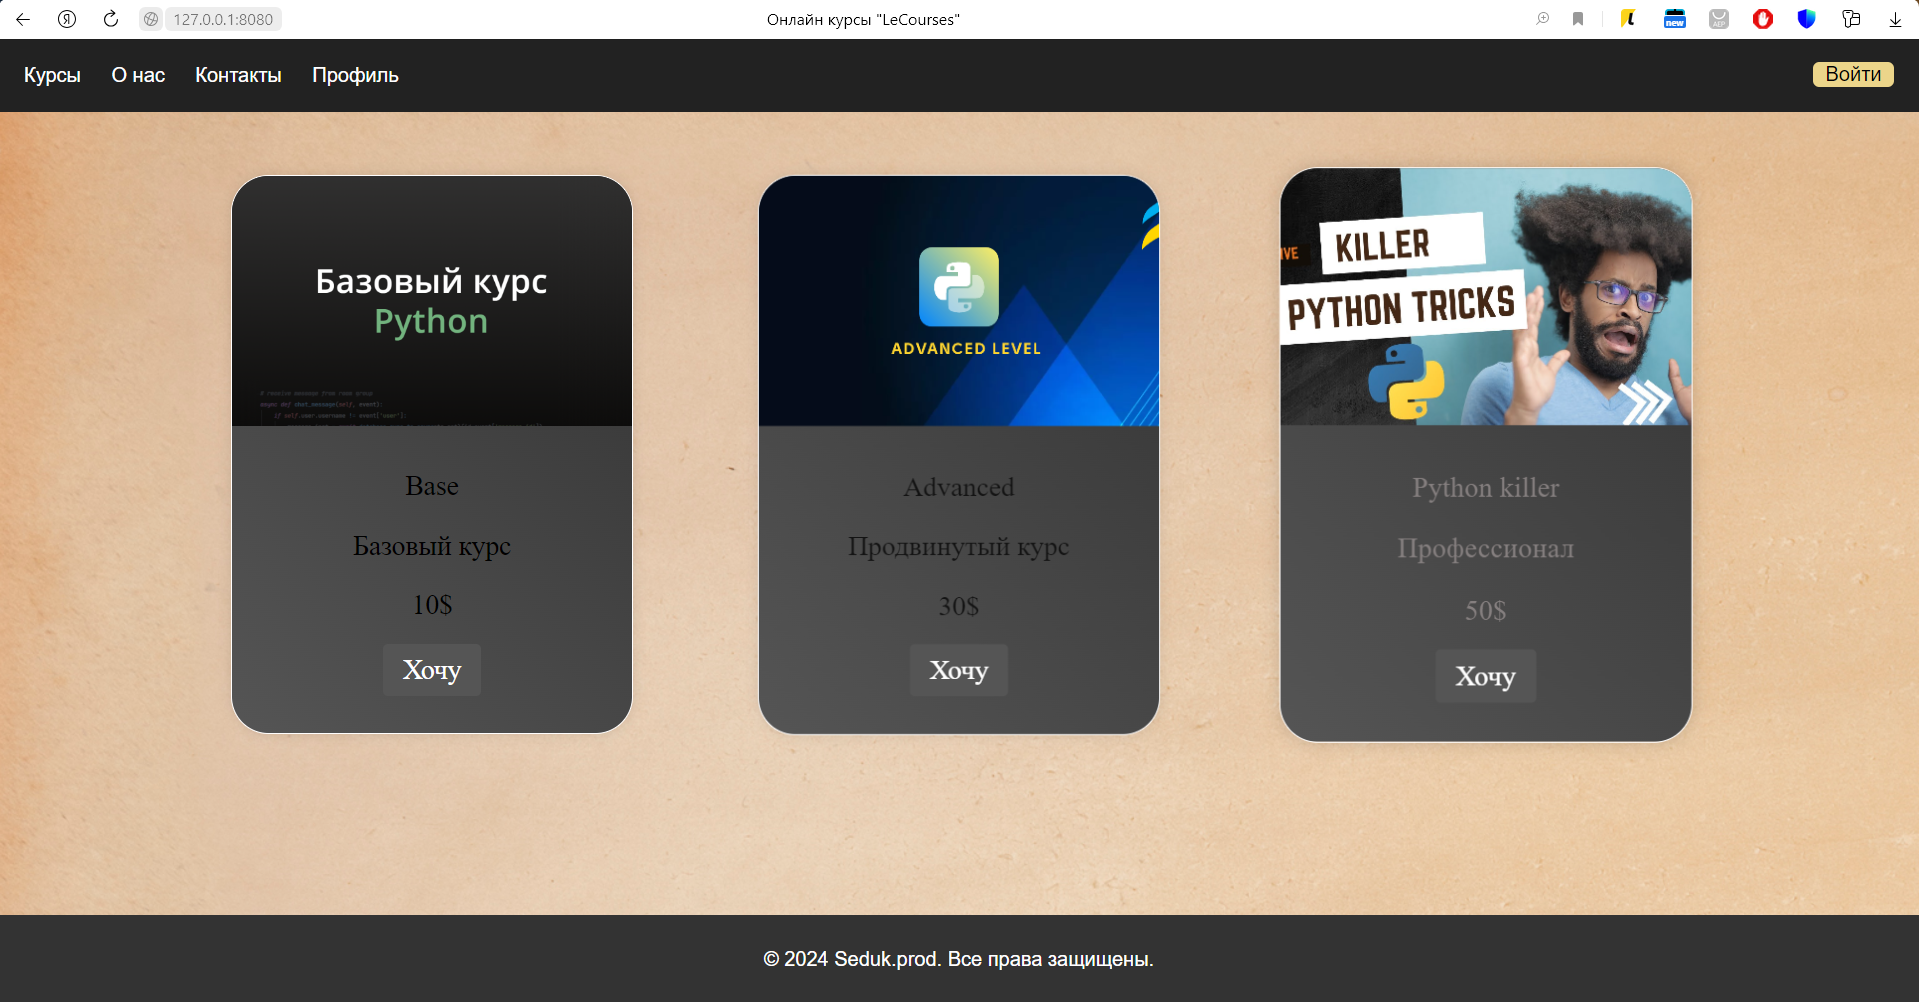
\includegraphics[width=1\linewidth]{main1}}
\center{\includegraphics[width=1\linewidth]{main2}}
\center{\includegraphics[width=1\linewidth]{main3}}
\caption{Главная страница сайта «Русатом – Аддитивные технологии»}
\label{main:image}
\end{figure}

На рисунке \ref{menu:image} представлен динамический вывод заголовков, включающий в себя искомые фразы при поиске фраз.

\begin{figure}[ht]
\center{
\includegraphics[width=1\linewidth]{menu}}
\caption{Динамический вывод заголовков}
\label{menu:image}
\end{figure}

На рисунке \ref{enter:image} представлен ввод данных для публикации новости.

\begin{figure}[ht]
\center{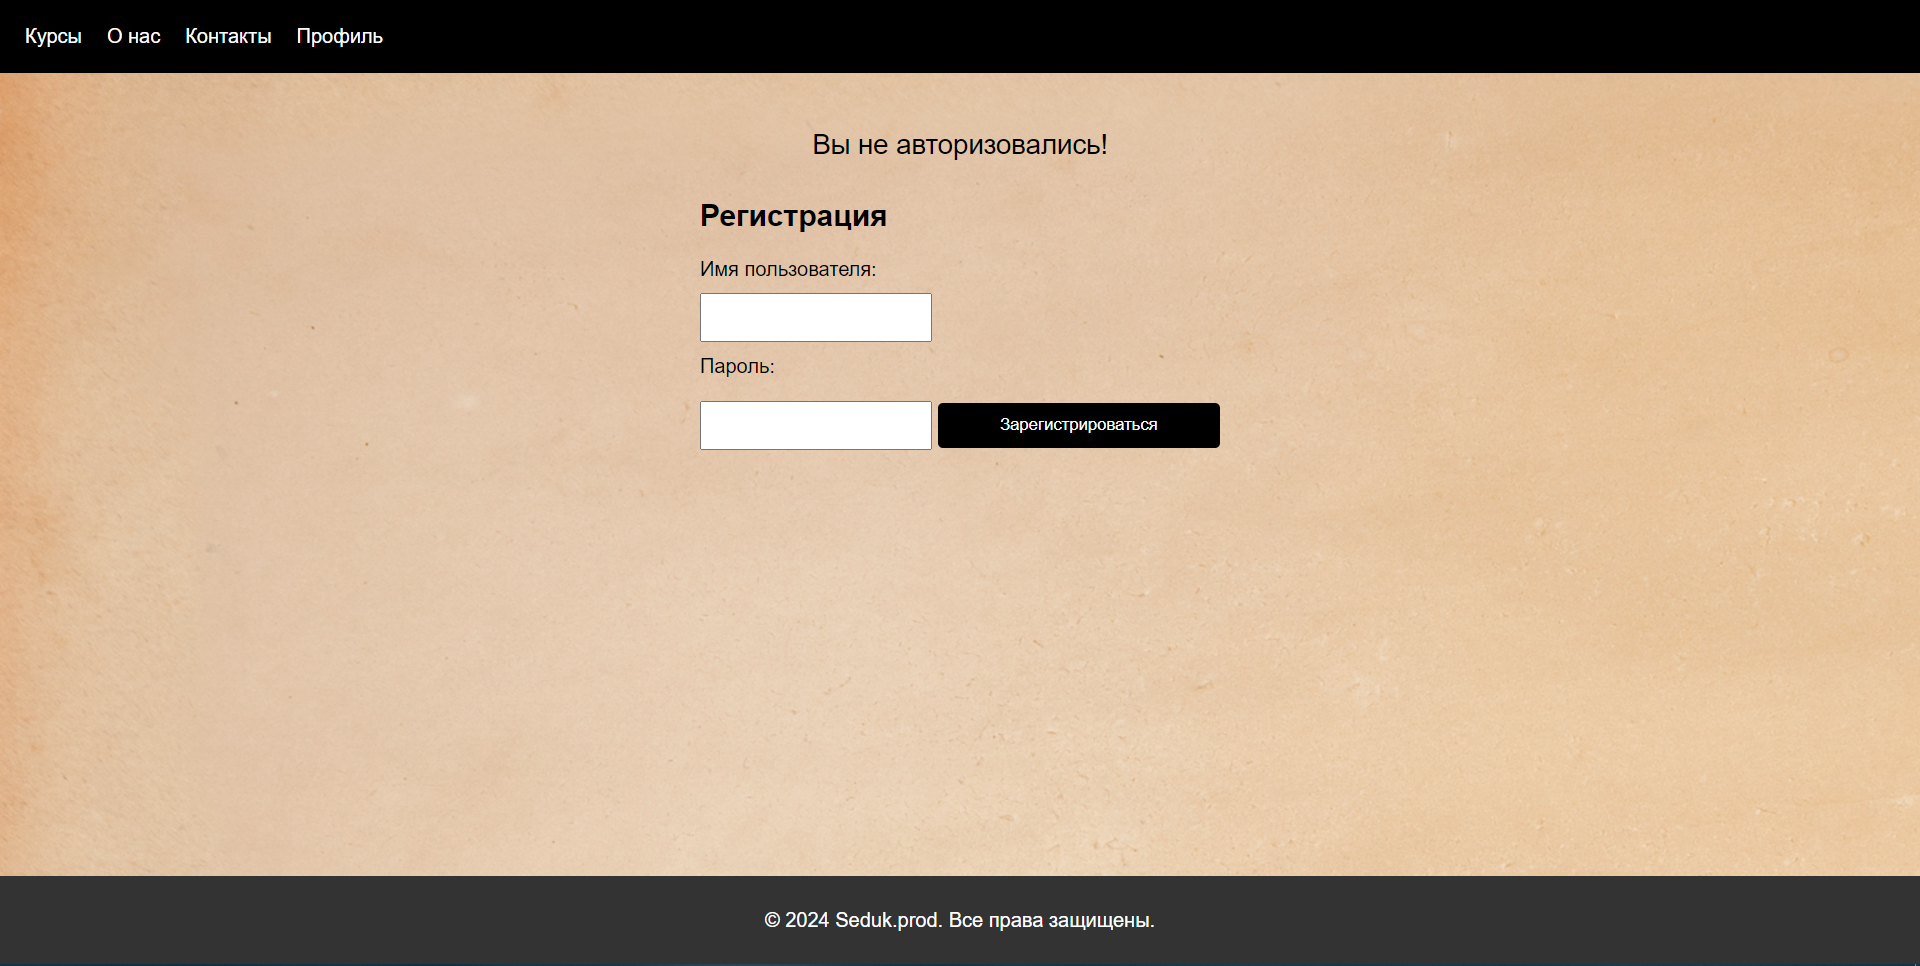
\includegraphics[width=1\linewidth]{enter}}
\caption{Ввод данных для публикации очень-очень длинной, интересной и полезной новости}
\label{enter:image}
\end{figure}

   \section*{ЗАКЛЮЧЕНИЕ}
\addcontentsline{toc}{section}{ЗАКЛЮЧЕНИЕ}

Преимущества аддитивных технологий заключается в разнообразии процессов, позволяющих применять их в различных областях производства. Существенным ограничением же является и экономическая составляющая, которая не позволит внедрить аддитивное производство повсеместно.
  
Компании, видя, как развиваются информационные технологии, пытаются использовать их выгодно для своего бизнеса, запуская свой сайт для того, чтобы заявить о своем существовании, проинформировать потенциального клиента об услугах или продуктах, которые предоставляет. 
Для продвижения компании «Русатом – Аддитивные технологии» был разработан веб-сайт на основе системы «1С-Битрикс: Управление сайтом».

Основные результаты работы:

\begin{enumerate}
\item Проведен анализ предметной области. Выявлена необходимость использовать 1С-Битрикс.
\item Разработана концептуальная модель web-сайта. Разработана модель данных системы. Определены требования к системе.
\item Осуществлено проектирование web-сайта. Разработана архитектура серверной части. Разработан пользовательский интерфейс web-сайта.
\item Реализован и протестирован web-сайт. Проведено модульное и системное тестирование.
\end{enumerate}

Все требования, объявленные в техническом задании, были полностью реализованы, все задачи, поставленные в начале разработки проекта, были также решены.

Готовый рабочий проект представлен адаптивной версткой сайта. Сайт находится в публичном доступе, поскольку опубликован в сети Интернет.  

}\fi
\addcontentsline{toc}{section}{СПИСОК ИСПОЛЬЗОВАННЫХ ИСТОЧНИКОВ}

\begin{thebibliography}{9}

    \bibitem{pip} Документация по Python [Электронный ресурс]. — Режим доступа: https://docs.python.org/3/.
    \bibitem{pip} Вигерс, К. Разработка требований к программному обеспечению : [практические приёмы сбора требований и управления ими при разработке программных продуктов : пер. с англ.] / К. Вигерс, Д. Битти. – 3-е изд., доп. – Санкт-Петербург : BHV, 2020. – 736 с. – ISBN 978-5-9775-3348-5. – Текст~: непосредственный.
	\bibitem{html5}	Голдстайн, А. HTML5 и CSS3 для всех / А. Голдстайн, Л. Лазарис, Э. Уэйл. – Москва~: Вильямс, 2012. – 368 с. – ISBN 978-5-699-57580-0. – Текст~: непосредственный.
	\bibitem{htmlcss} Дэкетт, Д. HTML и CSS. Разработка и создание веб-сайтов / Д. Дэкетт. – Москва~: Эксмо, 2014. – 480 с. – ISBN 978-5-699-64193-2. – Текст~: непосредственный.
	\bibitem{uchiru} Лоусон, Б. Изучаем HTML5. Библиотека специалиста / Б. Лоусон, Р. Шарп. – Санкт-Петербург : Питер, 2013 – 286 с. – ISBN 978-5-459-01156-2. – Текст~: непосредственный.
	\bibitem{bigbook} Макфарланд, Д. Большая книга CSS / Д. Макфарланд. – Санкт-Петербург : Питер, 2012. – 560 с. – ISBN 978-5-496-02080-0. – Текст~: непосредственный.
	\bibitem{1231} Павловская Т.А. Программирование на языке высокого уровня: Учебник для вузов / Т.А. Павловская. – СПб: "Издательский дом ""Питер""", 2021. – 432 с. ISBN 978-5-39583-497-9 – Текст~: непосредственный.  
	\bibitem{chaynik} Титтел, Э. HTML5 и CSS3 для чайников / Э. Титтел, К. Минник. – Москва~: Вильямс, 2016 – 400 с. – ISBN 978-1-118-65720-1. – Текст~: непосредственный.    
	\bibitem{22} Титтел, Э. HTML5 и CSS3 для чайников / Э. Титтел, К. Минник. – Москва~: Вильямс, 2016 – 400 с. – ISBN 978-1-118-65720-1. – Текст~: непосредственный.        
	\bibitem{servsssds}	Титтел, Э. HTML5 и CSS3 для чайников / Э. Титтел, К. Минник. – Москва~: Вильямс, 2016 – 400 с. – ISBN 978-1-118-65720-1. – Текст~: непосредственный.
	\bibitem{mysql}	Федоров, Д. Ю.  Программирование на языке высокого уровня Python : учебное пособие для прикладного бакалавриата / Д. Ю. Федоров. – 2-е изд., перераб. и доп. – Москва : Издательство Юрайт, 2019. – 161 с. – (Бакалавр. Прикладной курс). – ISBN 978-5-534-10971-9.  – Текст~: непосредственный.
	\bibitem{javascript} Фримен, А. Практикум по программированию на JavaScript / А. Фримен. – Москва~: Вильямс, 2013. – 960 с. – ISBN 978-5-8459-1799-7. – Текст~: непосредственный.
\end{thebibliography}

\ifВКР{\appendix{Представление графического материала}

Графический материал, выполненный на отдельных листах,
изображен на рисунках А.1--А.\arabic{числоПлакатов}.
\setcounter{числоПлакатов}{0}

\renewcommand{\thefigure}{А.\arabic{figure}} % шаблон номера для плакатов

\begin{landscape}

\begin{плакат}
    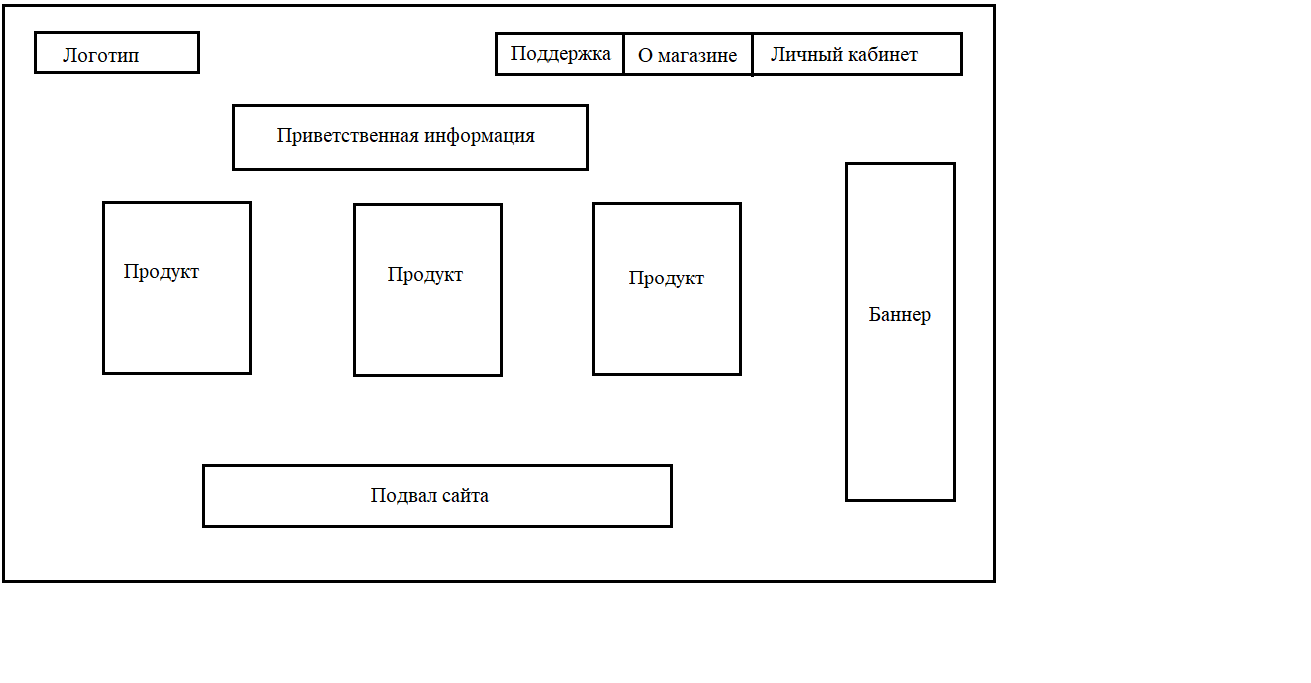
\includegraphics[width=0.82\linewidth]{плакат1.png}
    \заголовок{Сведения о ВКРБ}
    \label{pl1:image}      
\end{плакат}

\begin{плакат}
    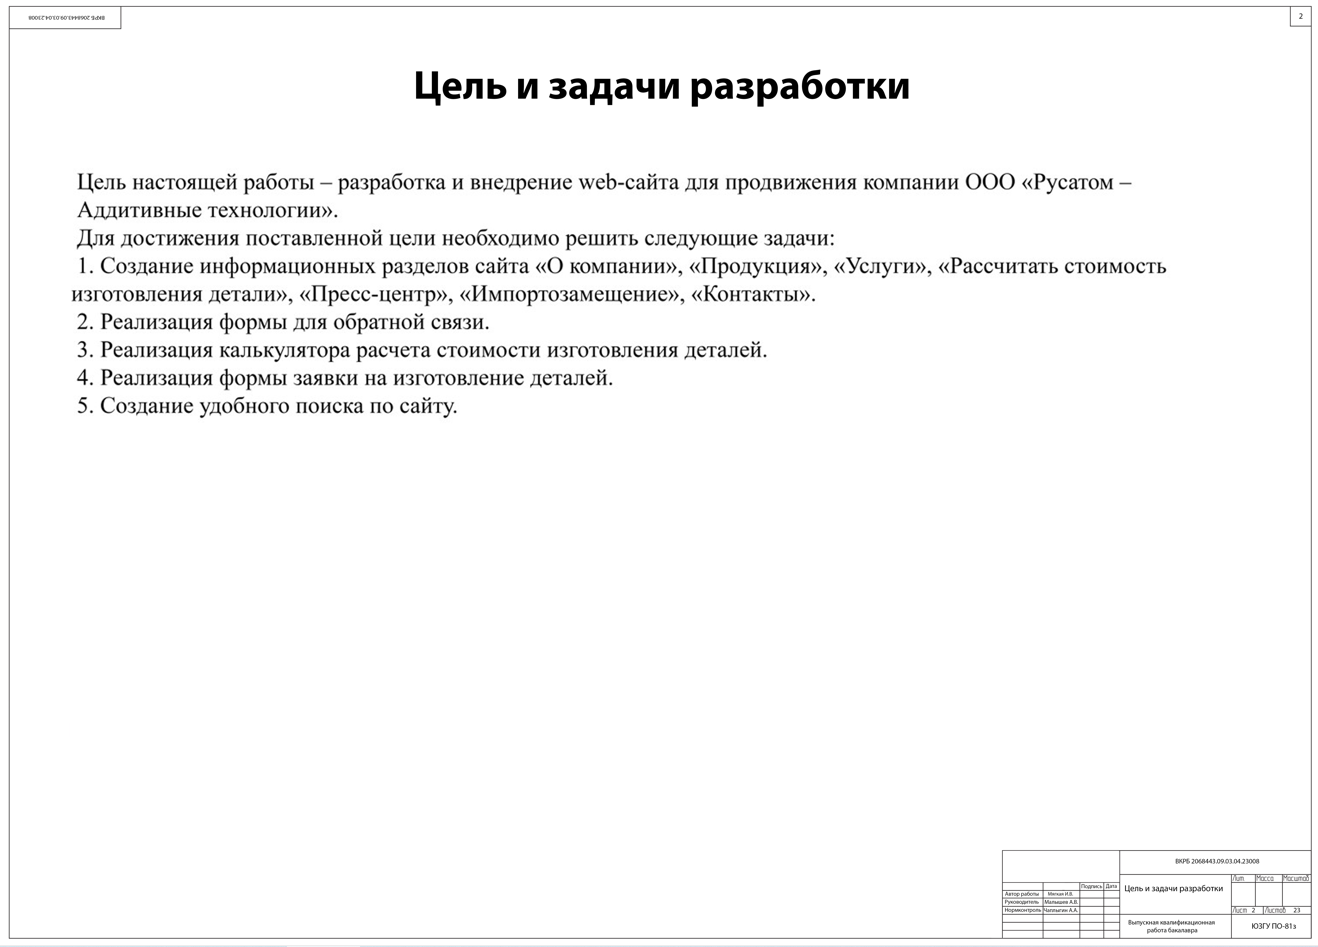
\includegraphics[width=0.82\linewidth]{плакат2.png}
    \заголовок{Цель и задачи разработки}
    \label{pl2:image}      
\end{плакат}

\begin{плакат}
    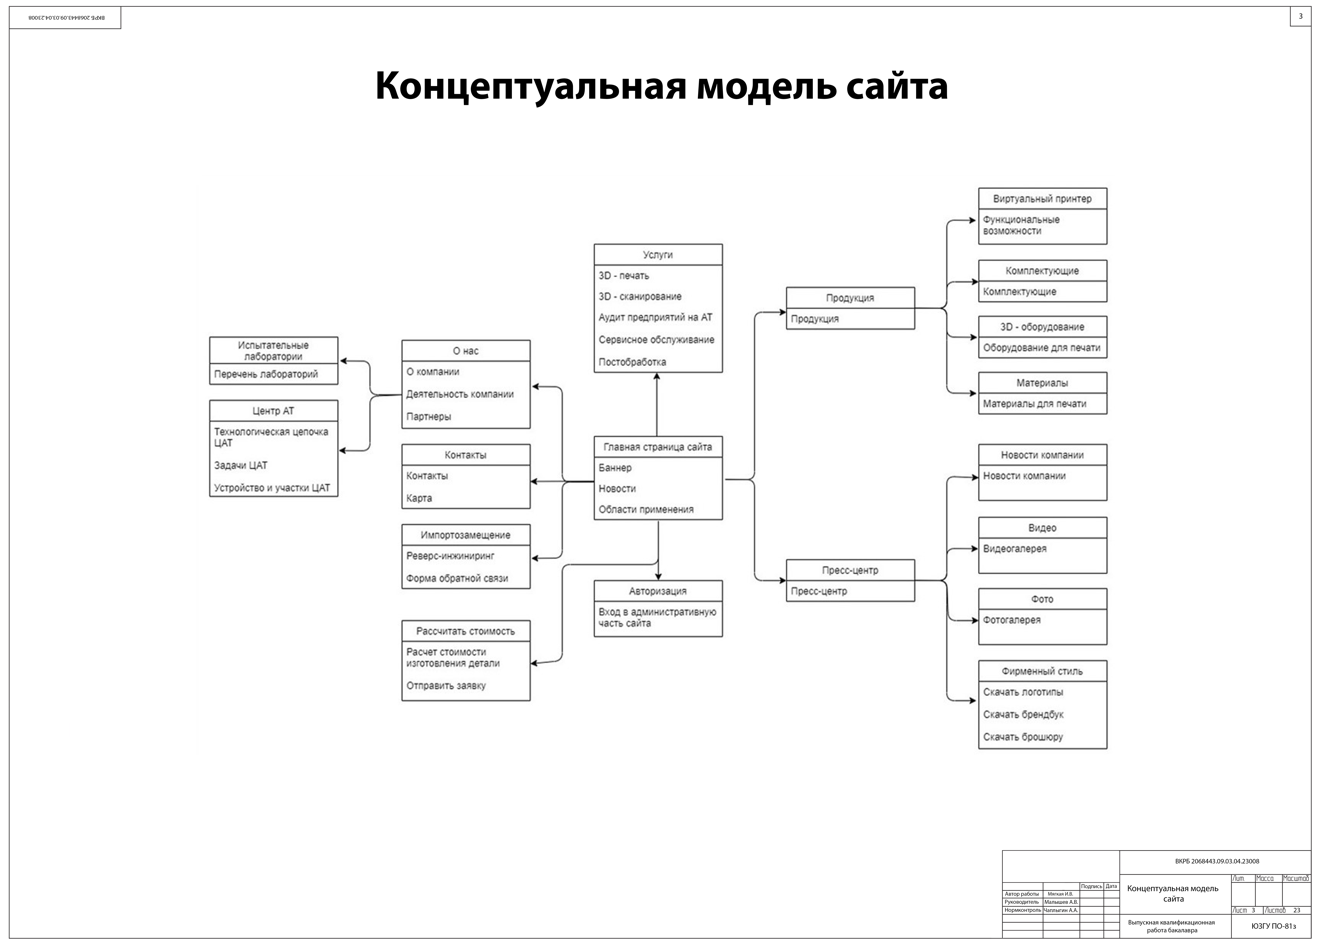
\includegraphics[width=0.82\linewidth]{плакат3.png}
    \заголовок{Концептуальная модель сайта}
    \label{pl3:image}      
\end{плакат}

\begin{плакат}
    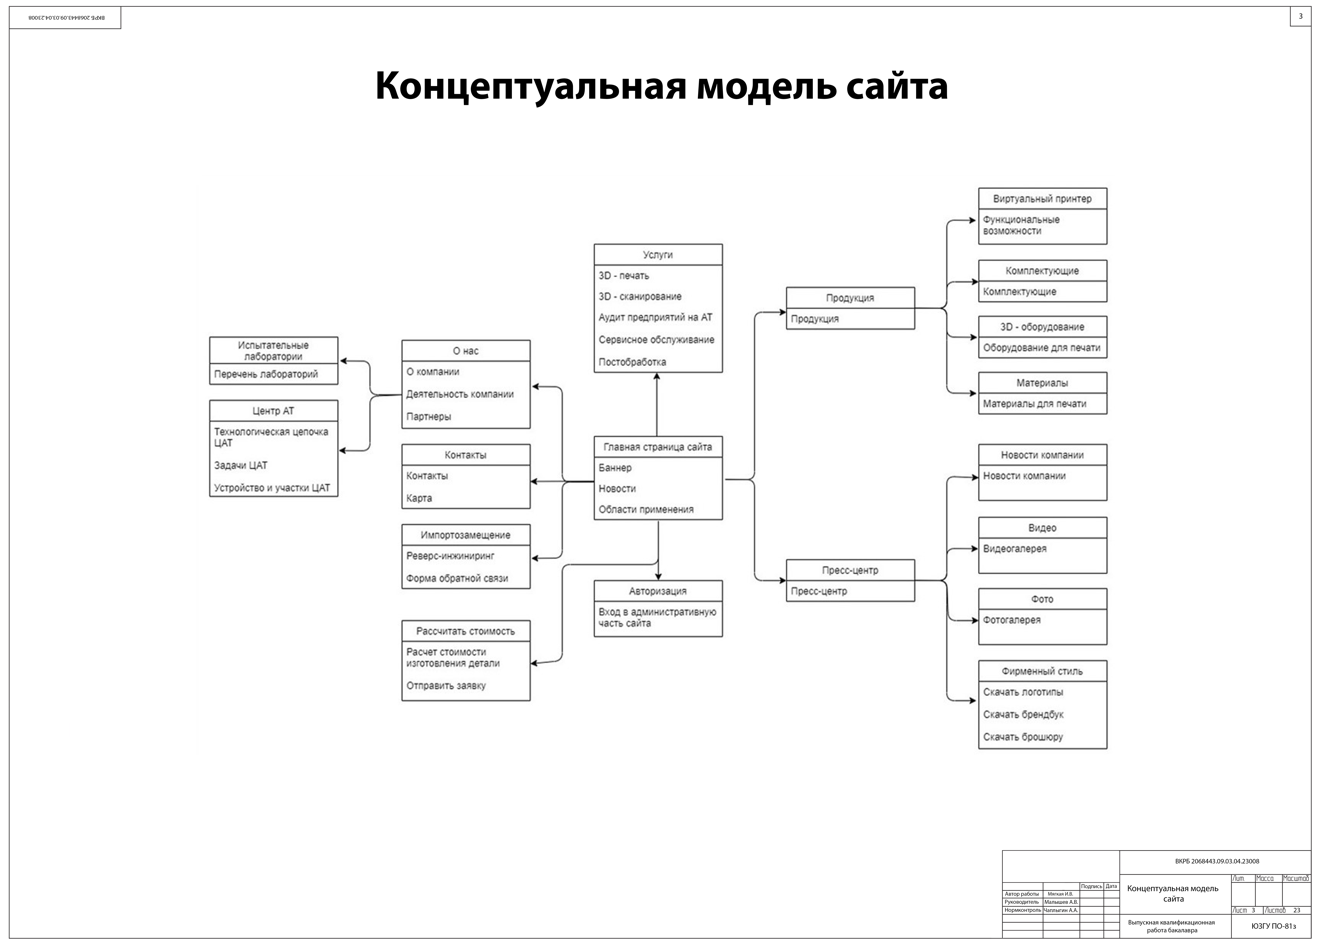
\includegraphics[width=0.82\linewidth]{плакат3.png}
    \заголовок{Еще плакат}
    \label{pl4:image}      
\end{плакат}

\end{landscape}
}\fi
\ifПрактика{}\else{\appendix{Фрагменты исходного кода программы}

server.py
\lstinputlisting[language=Python, frame=none]{kod/server.py}

serve\_file.py
\lstinputlisting[language=Python, frame=none]{kod/serve_file.py}

dump\_db.py
\lstinputlisting[language=Python, frame=none]{kod/dump_db.py}

render\_template.py
\lstinputlisting[language=Python, frame=none]{kod/render_template.py}

base\_view.py
\lstinputlisting[language=Python, frame=none]{kod/base_view.py}

home\_view.py
\lstinputlisting[language=Python, frame=none]{kod/home_view.py}

user\_view.py
\lstinputlisting[language=Python, frame=none]{kod/user_view.py}

payment\_view.py
\lstinputlisting[language=Python, frame=none]{kod/payment_view.py}

login\_view.py
\lstinputlisting[language=Python, frame=none]{kod/login_view.py}

courses\_view.py
\lstinputlisting[language=Python, frame=none]{kod/courses_view.py}

contact\_us\_view.py
\lstinputlisting[language=Python, frame=none]{kod/contact_us_view.py}


\ifВКР{
	\newpage
	\addcontentsline{toc}{section}{На отдельных листах (CD-RW в прикрепленном конверте)}
	\begin{center}
		\textbf{Место для диска}
	\end{center}
}\fi}\fi
\end{document}
